\section{Ground Truth}\label{sec:ground-truth}
In this section, we introduce our ground truth to establish that both black-box analysis 
and white-box analysis can analyze simple, configurable systems and identify weaknesses. 

To do so, we design multiple configurable systems that test both analyses in different scenarios. 
Afterward, we evaluate as described in \autoref{ch:operationalization}. 
Since we design these systems ourselves, we have a baseline from which we manually build the {\perfInfluenceModel}s that we use for comparison. 
We design all these systems with a different focus in mind, such as a system that includes multicollinearity, 
to see to what extent they influence the analyses. 

Each system uses \emph{Simple Interaction} as the base system, however, they extend or change the system in different ways.

\paragraph{Simple Interaction}\label{ground-truth:Simple}
For our first system, we use the code from our previous example in \autoref{lst:performanceExample} and provide an additional feature model 
of the system in \autoref{fig:feature_abcd}. 
Since we use this as our base system, extending as needed to fit each
particular scenario, it is kept intentionally simple, only containing some interactions and no constraints.

\begin{figure}[h]
    \centering
    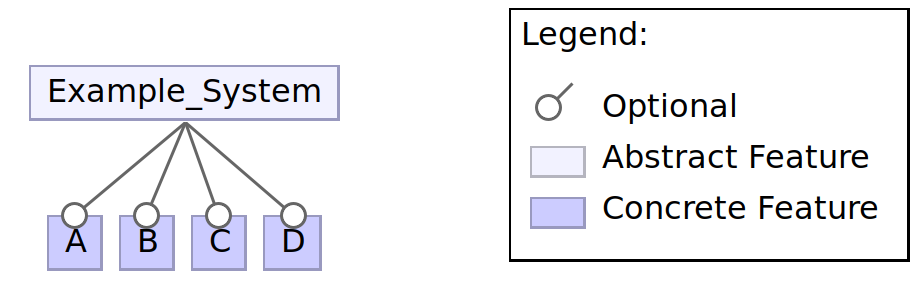
\includegraphics[scale=0.25]{gfx/Feature_ABCD.png}
    \caption{Feature model of \autoref{lst:performanceExample}.}
    \label{fig:feature_abcd}
\end{figure}


\paragraph{Else Clause}
The first modification is the addition of an \emph{else clause} to the if statement of feature \emph{A} in \autorefLine{line:feature_A_statement}. 
We encode this as follows:

\begin{minipage}{\linewidth}
    \begin{lstlisting}[language=C++,label={lst:else_case},escapechar=|]
if(A)
    fpcsc::sleep_for_secs(1); 
else
    fpcsc::sleep_for_secs(2);
    \end{lstlisting}
    \end{minipage}

We expect the white-box analysis to attribute the time spent in the \emph{else clause} to feature \emph{A} 
since it is a part of the feature region of feature \emph{A}. 
In contrast, 
the black-box analysis cannot differentiate between the \emph{else clause} that is executed when feature \emph{A} is unselected and the time spent in \emph{Base}.

\paragraph{Function}\label{ground-truth:Function}
Another modification of our \emph{Simple Interaction} system is adding a function in which we spend time. 
In \autorefLine{line:feature_A} we call the function \emph{waste\_time(1)} instead of \emph{fpcsc::sleep\_for\_secs(1)}.

\begin{minipage}{\linewidth}
\begin{lstlisting}[language=C++,label={lst:function},escapechar=|]
void waste_time(int duration){
    fpcsc::sleep_for_secs(duration);
}
\end{lstlisting}
\end{minipage}

Both white-box and black-box analysis should be able to still correctly attribute the time spent in each feature.

\paragraph{Multicollinearity}\label{ground-truth:Multicollinearity}
Instead of modifying the system's code, we add a restriction to the feature model of \autoref{fig:feature_abcd}. 
We change feature \emph{B} from optional to mandatory, this changes the feature model and 
introduces multicollinearity into the system. 
We see the modified in \autoref{fig:multicollinearity}.
The white-box analysis should still be able to correctly identify the time spent in \emph{Base} and feature \emph{B}, 
while the black-box analysis should distribute the time spent between the features differently.

\begin{figure}[h]
    \centering
    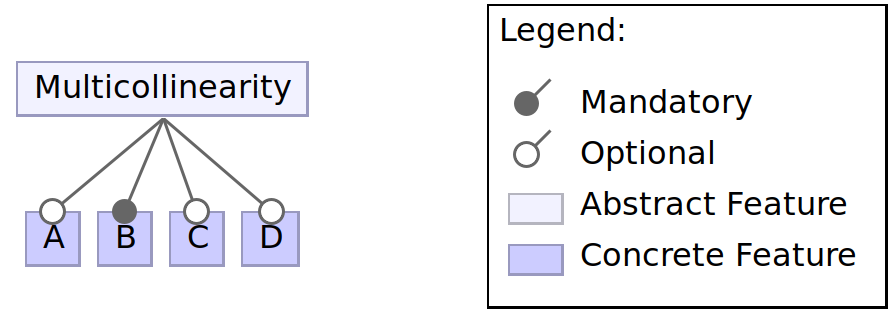
\includegraphics[scale=0.25]{gfx/Multicollinearity.png}
    \caption{Feature model of the \emph{Multicollinearity} system.}
    \label{fig:multicollinearity}
\end{figure}

\paragraph{Shared Feature Variable}\label{ground-truth:Shared}
We now add an optional feature \emph{E} to the system. 
However, instead of encoding it like the previous features by specifying a separate variable, 
we modify the feature variable \emph{D} in \autorefLine{line:feature_declatation} to a \texttt{string de = "00"} 
for which the first character represents feature \emph{D} and the second character \emph{E}. If either is selected, 
we assign the character for that feature \emph{"1"}. We add another \emph{if statement} to spend time if \emph{E} is selected and encode this as follows:

\begin{minipage}{\linewidth}
\begin{lstlisting}[language=C++,label={lst:shared},escapechar=|]
std::string de = "00";

if(de[0] == '1')
    fpcsc::sleep_for_secs(2);

if(de[1] == '1')
    fpcsc::sleep_for_secs(1);
\end{lstlisting}
\end{minipage}

We expect the black-box analysis to still work as intended, but the white-box analysis to be inaccurate since both features \emph{D} and \emph{E} share the same feature variable. 
Each feature region of \emph{D} or \emph{E} should now be influenced by the feature interaction \emph{\{D, E\}}.